%%%%%%%%%%%%%%%%%%%%% PACKAGE IMPORTS %%%%%%%%%%%%%%%%%%%%%
\documentclass{article}
\usepackage{import}

\usepackage{amsmath, amsfonts, amsthm, amssymb}
\usepackage{lmodern}
\usepackage{microtype}
\usepackage{fullpage}       
\usepackage{changepage}
\usepackage{hyperref}
\usepackage{blindtext}
\hypersetup{
    colorlinks=true,
    linkcolor=blue,
    filecolor=magenta,      
    urlcolor=blue,
    pdftitle={Overleaf Example},
    pdfpagemode=FullScreen,
    }
\urlstyle{same}

\newenvironment{level}%
{\addtolength{\itemindent}{2em}}%
{\addtolength{\itemindent}{-2em}}

\usepackage{amsmath,amsthm,amssymb}

\usepackage[nooldvoltagedirection]{circuitikz}
\usetikzlibrary{decorations,arrows,shapes}

\usepackage{datetime}
\usepackage{etoolbox}
\usepackage{enumerate}
\usepackage{enumitem}
\usepackage{listings}
\usepackage{array}
\usepackage{varwidth}
\usepackage{tcolorbox}
\usepackage{amsmath}
\usepackage{circuitikz}
\usepackage{verbatim}
\usepackage[linguistics]{forest}
\usepackage{listings}
\usepackage{xcolor}
\renewcommand{\rmdefault}{cmss}


\newcommand\doubleplus{+\kern-1.3ex+\kern0.8ex}
\newcommand\mdoubleplus{\ensuremath{\mathbin{+\mkern-10mu+}}}

\definecolor{codegreen}{rgb}{0,0.6,0}
\definecolor{codegray}{rgb}{0.5,0.5,0.5}
\definecolor{codepurple}{rgb}{0.58,0,0.82}
\definecolor{backcolour}{rgb}{0.95,0.95,0.92}

\lstdefinestyle{mystyle}{
    language=Python,
    basicstyle=\ttfamily\small,
    keywordstyle=\color{blue},
    stringstyle=\color{red},
    commentstyle=\color{green},
    morecomment=[l][\color{magenta}]{\#},
    backgroundcolor=\color{backcolour},   
    breakatwhitespace=false,         
    breaklines=true,                 
    captionpos=b,                    
    keepspaces=true,                 
    numbers=left,                    
    numbersep=5pt,                  
    showspaces=false,                
    showstringspaces=false,
    showtabs=false,                  
    tabsize=2
}

\lstset{style=mystyle}
\setlength{\parindent}{0pt}
\setlength{\parskip}{5pt plus 1pt}

\providetoggle{questionnumbers}
\settoggle{questionnumbers}{true}
\newcommand{\noquestionnumbers}{
    \settoggle{questionnumbers}{false}
}

\newcounter{questionCounter}
\newenvironment{question}[2][\arabic{questionCounter}]{%
    \ifnum\value{questionCounter}=0 \else {\newpage}\fi%
    \setcounter{partCounter}{0}%
    \vspace{.25in} \hrule \vspace{0.5em}%
    \noindent{\bf \iftoggle{questionnumbers}{Question #1: }{}#2}%
    \addtocounter{questionCounter}{1}%
    \vspace{0.8em} \hrule \vspace{.10in}%
}

\newcounter{partCounter}[questionCounter]
\renewenvironment{part}[1][\alph{partCounter}]{%
    \addtocounter{partCounter}{1}%
    \vspace{.10in}%
    \begin{indented}%
       {\bf (#1)} %
}{\end{indented}}

\def\indented#1{\list{}{}\item[]}
\let\indented=\endlist
\def\show#1{\ifdefempty{#1}{}{#1\\}}
\def\IMP{\longrightarrow}
\def\AND{\wedge}
\def\OR{\vee}
\def\BI{\leftrightarrow}
\def\DIFF{\setminus}
\def\SUB{\subseteq}


\newcolumntype{C}{>{\centering\arraybackslash}m{1.5cm}}
\renewcommand\qedsymbol{$\blacksquare$}
\newtcolorbox{answer}
{
  colback   = green!5!white,    % Background colorucyitc,
  colframe  = green!75!black,   % Outline color
  box align = center,           % Align box on text line
  varwidth upper,               % Enables multi line input
  hbox                          % Bounds box to text width
}

\newcommand{\myhwname}{CSE 447 Assignment 1}
\newcommand{\myname}{Sebastian Liu}
\newcommand{\myemail}{ll57@cs.washington.edu}
\newcommand{\mysection}{AB}
\newcommand{\dollararrow}{\stackrel{\$}{\leftarrow}}
%%%%%%%%%%%%%%%%%%%%%%%%%%%%%%%%%%%%%%%%%%%%%%%%%%%%%%%%%%%

%%%%%%%%%%%%%%%%%%% Document Options %%%%%%%%%%%%%%%%%%%%%%
\noquestionnumbers
%%%%%%%%%%%%%%%%%%%%%%%%%%%%%%%%%%%%%%%%%%%%%%%%%%%%%%%%%%%

%%%%%%%%%%%%%%%%%%%%%%%% WORK BELOW %%%%%%%%%%%%%%%%%%%%%%%%
\begin{document}

\begin{center}
    \textbf{Assignment 1} \bigskip
\end{center}

%%%%%%%%%%%%%%%%%%%%%%%% Task 1 %%%%%%%%%%%%%%%%%%%%%%%%M
\begin{question}{1.2 N-gram Language Modeling \& Perplexity (28\%)}
    \begin{part}
       \begin{answer}
        First, each line in the dataset are treated as a sequence. The sequence was tokenized using whitespace as the delimiter. Special tokens were added at the start (START) and end (STOP) of sequences.
        The vocabulary was built from the training data. Tokens appearing less than three times replaced by an (UNK) token. The final vocabulary size for the training set was 26,602.\\
         My unigram model was constructed by counting the frequency of each token in the training data. The (START) token is not considered since they don't influence the probability of unigrams. I calculated each token's probability base on its frequency relative to the total number of tokens.\\
         My bigram model was built by calculating the frequencies of pairs of consecutive tokens. I included bigrams starting with (START) token to get the beginning of sentences. I calculated the probabilities of bigrams as the frequency of the bigram divided by the frequency of its first token.\\
      The trigram model was similar to bigram expect we calculate the frequencies of triplets of consecutive tokens instead. The model includes trigrams that began with one or two (START) tokens. The probability of a trigram was calculated as the frequency of the trigram divided by the frequency of its first two tokens.\\
      All three models has an option to turn on laplace smoothing in which case we add 1 to each count and calculate the probabilities as the frequency of the n-gram plus 1 divided by the frequency of its first $n-1$ tokens plus the size of the vocabulary. \\
Model Sizes:
            \begin{tabular}{|c|c|}
                \hline
                \textbf{Model Type} & \textbf{Number of N-grams} \\
                    \hline
                    Unigram & 26,602 \\
                    \hline
                    Bigram & 510,391 \\
                    \hline
                    Trigram & 1,116,160 \\
                    \hline
            \end{tabular}
        \end{answer}

    \end{part}

    \begin{part}
        \begin{answer}
            Perplexity without smoothing was calculated as the following:

            \begin{equation}
                PPL(S) = \exp \left( -\frac{1}{|S|} \sum_{i=1}^{|S|} \log P(s_i | s_1,...,s_{i-1}) \right)
            \end{equation}

            Where:
            \begin{itemize}
                \item $PPL(S)$ is the perplexity of sequence $S$.
                \item $ P(s_i | s_1,...,s_{i-1})$ is the probability of token $s_i$ given its previous tokens $s_1,...,s_{i-1}$.
            \end{itemize}

            The final perplexity is calculated by taking the weighted average over all sequences (discounted by the number of words in each line):\\
            np.average(a\_list\_of\_perplexities, weights=a\_list\_of\_lengths).

         \end{answer}
     \end{part}
\newpage
     \begin{part}
        \begin{answer}
                Laplace smoothing disproportionately inflates the probabilities of n-grams with low probabilities.
                Since probabilities has to add up to 1, adding 1 counts to each n-grams effectively reduces the probabilities of more frequent n-grams,
                which might bias the model towards n-grams with low probabilities. \\

                \textbf{Empirical Evidence:}
                Comparing the perplexity scores of the training set with and without Laplace smoothing,
                we can see that the perplexity of the unigram model is relatively stable, but a significant
                increase is observed for the bigram and trigram models:
                \\\\
                \begin{tabular}{|c|c|c|}
                \hline
                \textbf{Model Type} & \textbf{Training Set Perplexity Unsmoothed} & \textbf{Training Set Perplexity Smoothed} \\
                \hline
                Unigram & 857.98 & 856.69  \\
                Bigram & 69.34 & 1268.06  \\
                Trigram & 6.36 & 4073.12 \\
                \hline
                \end{tabular}

         \end{answer}
     \end{part}

     \begin{part}
        \begin{answer}

             When \( k \) is small, model gives a high perplexity due to underestimating the probability of unseen N-grams.
             As \( k \) increases, the model starts giving lower perplexities, when values of \( k \) approaching 1
             the model starts to increase perplexity again.

            Seems like there's a non-linear relationship between \( k \) and perplexity, with an optimal range where the perplexity is minimized.
            I believe this is related to bias and variance tradeoff, where we need to use empirical methods to find the optimal value of \( k \).
         \end{answer}
     \end{part}

     \begin{part}
        \begin{answer}

            The perplexity scores for unigram, bigram, and trigram models describe the performance of the models in predicting the sequences in the dataset.

            \textbf{Perplexity without Smoothing:}
            \begin{tabular}{|c|c|c|c|}
            \hline
            \textbf{Model Type} & \textbf{Training Set} & \textbf{Development Set} & \textbf{Test Set} \\
            \hline
            Unigram & 857.98 & 786.03 & 790.21 \\
            Bigram & 69.34 & Infinity & Infinity \\
            Trigram & 6.36 & Infinity & Infinity \\
            \hline
            \end{tabular}\\


            In the bigram and trigram models, when evaluated on the validation and test datasets, the perplexity reached an infinite value. This probably because the probability of some bigram/trigrams being zero. Given that no smoothing technique was applied in this instance, it is reasonable for the perplexity to be infinite.\\

            \textbf{Perplexity with Laplace Smoothing:}
            \begin{tabular}{|c|c|c|c|}
            \hline
            \textbf{Model Type} & \textbf{Training Set} & \textbf{Development Set} & \textbf{Test Set} \\
            \hline
            Unigram & 856.69 & 786.26 & 790.28 \\
            Bigram & 1268.06 & 1460.34 & 1459.36 \\
            Trigram & 4073.12 & 6389.98 & 6367.86 \\
            \hline
            \end{tabular}\\

            With Laplace smoothing, the perplexity of the unigram model remains relatively stable, but a significant increase is observed for the bigram and trigram models.
            It shows that Laplace smoothing resolves issues with unseen N-grams but, at the same time, may introduce inaccuracies in N-gram probabilities for higher-order models.
            Here we might be oversmoothing the bigram and trigram models, which gives to a much higher perplexity score after smoothing.
         \end{answer}
     \end{part}
\end{question}

%%%%%%%%%%%%%%%%%%%%%%%% Task 2 %%%%%%%%%%%%%%%%%%%%%%%%
\begin{question}{1.3 Interpolation (17\%)}
    \begin{part}
        \begin{answer}

                The goal was to minimize perplexity, which means a better predictive model.\\
                \textbf{Experiment Results:}

                \begin{tabular}{|c|c|c|c|c|c|}
                \hline
                \(\lambda_1\) & \(\lambda_2\) & \(\lambda_3\) & Training Perplexity & Dev Perplexity & Test Perplexity \\
                \hline
                0.33 & 0.33 & 0.34 & 15.97 & 373.73 & 376.34 \\
                0.2 & 0.3 & 0.5 & 12.07 & 440.87 & 444.20 \\
                0.2 & 0.2 & 0.6 & 10.79 & 495.22 & 498.82 \\
                0.1 & 0.15 & 0.75 & 9.09 & 689.24 & 695.13 \\
                0.05 & 0.08 & 0.87 & 8.16 & 1095.98 & 1107.03 \\
                0.1 & 0.3 & 0.6 & 10.45 & 550.59 & 555.71 \\
                \hline
                \end{tabular}\\


                The strategy is gradually shifting the weight from unigram towards bigram and trigram models.
                Since the weight on higher-order n-grams increased, we see a general trend of reduced training perplexity
                but development and test perplexity increased. Meaning that higher-order
                n-grams are more predictive on training data, but they may overfit unseen data.

         \end{answer}
     \end{part}

     \begin{part}
        \begin{answer}

            The optimal combination of hyperparameters are chosen based on their lowest perplexity on the development set.

            \textbf{Optimal Hyperparameters:}
\( \lambda_1 = 0.33 \),
 \( \lambda_2 = 0.33 \),
 \( \lambda_3 = 0.34 \)


            \textbf{Perplexity on Test Set:} 376.34

         \end{answer}
     \end{part}
\newpage
     \begin{part}
        \begin{answer}

            With half the training data, I would expect the perplexity to decrease. Because in my implementation, I replace unseen words with UNK tokens, when
            we reduce the training data, we would expect to see a lot more UNK tokens which gives a more general model (less variety in vocabulary). When evaluating
            on the dev and test set we would have a lower perplexity.\\

            \textbf{Empirical Evidence:}
            In the experiment, I deleted half of the training data. We can see compare to the perplexities in part (a), the perplexities on the dev and
            test sets decreased. \\

            \begin{tabular}{|c|c|c|c|c|c|}
                \hline
                \(\lambda_1\) & \(\lambda_2\) & \(\lambda_3\) & Training Perplexity & Dev Perplexity & Test Perplexity \\
                \hline
                0.33 & 0.33 & 0.34 & 13.37 & 352.93 & 354.31 \\
                0.2 & 0.3 & 0.5 & 10.09 & 424.28 & 425.62 \\
                0.2 & 0.2 & 0.6 & 9.01 & 477.04 & 478.78 \\
                0.1 & 0.15 & 0.75 & 7.58 & 677.62 & 679.66 \\
                0.05 & 0.08 & 0.87 & 6.81 & 1096.53 & 1099.77 \\
                0.1 & 0.3 & 0.6 & 8.74 & 541.30 & 542.30 \\
                \hline
                \end{tabular}\\


         \end{answer}
     \end{part}

     \begin{part}
        \begin{answer}

            Increasing this threshold (from tokens appearing three times to those appearing less than five times) increases the number of UNK tokens,
            making the model more general and potentially less sensitive to changes in the language.

            \textbf{Empirical Evidence:}
            In my experiments, increasing the UNK threshold to 5 gives a decrease in perplexity across, dev and test sets (compare to part(a)).

            \begin{tabular}{|c|c|c|c|c|c|}
                \hline
                \(\lambda_1\) & \(\lambda_2\) & \(\lambda_3\) & Training Perplexity & Dev Perplexity & Test Perplexity \\
                \hline
                0.33 & 0.33 & 0.34 & 17.25 & 306.39 & 308.06 \\
                0.2 & 0.3 & 0.5 & 13.15 & 354.99 & 357.06 \\
                0.2 & 0.2 & 0.6 & 11.80 & 398.27 & 400.44 \\
                0.1 & 0.15 & 0.75 & 9.99 & 542.14 & 545.59 \\
                0.05 & 0.08 & 0.87 & 9.00 & 844.17 & 850.43 \\
                0.1 & 0.3 & 0.6 & 11.43 & 433.26 & 436.39 \\
                \hline
                \end{tabular}\\
         \end{answer}
     \end{part}

\end{question}

%%%%%%%%%%%%%%%%%%%%%%%% Task 3 %%%%%%%%%%%%%%%%%%%%%%%%
\begin{question}{2 Byte-Pair Encoding (BPE) (30\%) }
    \begin{part}
        \begin{answer}
                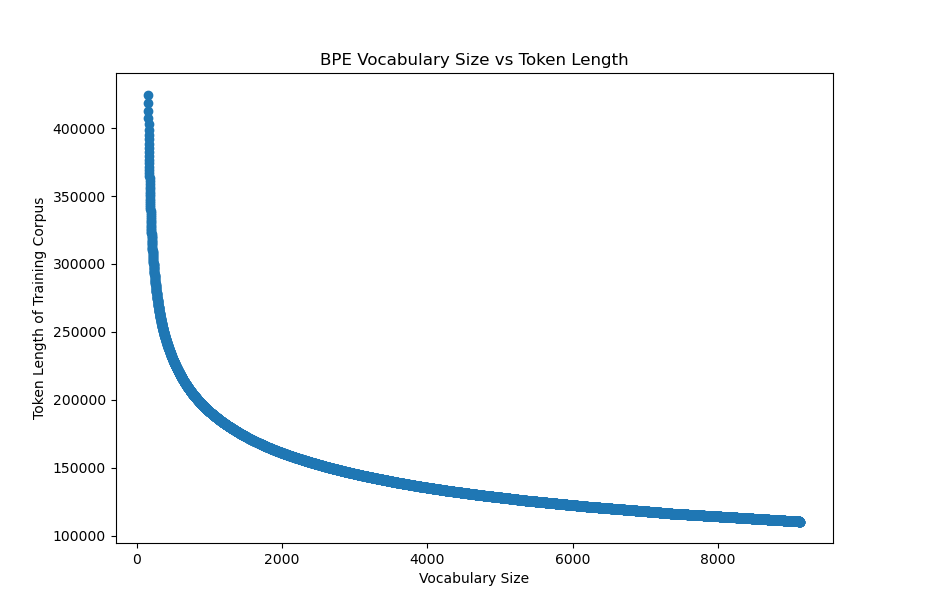
\includegraphics[width=1\textwidth]{../scatter.png}

                The final vocabulary size after training the BPE tokenizer is \textbf{9124} types.
                The total length of the training data under the final type vocabulary is \textbf{110469}.

        \end{answer}
     \end{part}

     \begin{part}
        \begin{answer}
            Character-level encoding has no out-of-vocabulary issues and can be more generally applied to text with different contents.
            However, breaking sequences into characters gives longer sequences and
            also loses the semantic context (e.g. "happy" and "ppahy" made up by the same token, one makes sense to human
            but the other one doesn't).
            BPE, however, gives a more balance solution between OOV issues and semantic context.
            Because it creates a vocabulary of subword units, instead of single characters, from frequent bigrams in the
            training data. BPE, compare to character-level encoding, reduces sequence length and maintains more semantic information, but
            its performance can be heavily dependent on the representativeness of the training corpus (e.g. if the training corpus is trained on
            computer science papers, it might not perform well on medical papers).

        \end{answer}
     \end{part}
\newpage
     \begin{part}
        \begin{answer}
            1. Applying the trained BPE tokenizer on the last 1000 lines of the dataset gave a total of \textbf{30126} tokens.\\
            2. The tokenizer seems to be able to handle unseen words
            by breaking them down to smaller known units, which might be why the total number of tokens is relatively quite high.\\
            3. In general, I expect the BPE tokenizer to perform reasonably well on texts that are similar to its training corpus.
            I would expect my tokenizer to fail on texts that are very different from the training corpus, such as domain-specific texts
            that contains a lot of special terms that are not in the training corpus.

        \end{answer}
     \end{part}
\end{question}

%%%%%%%%%%%%%%%%%%%%%%%% Task 4 %%%%%%%%%%%%%%%%%%%%%%%%
\begin{question}{3 WordPiece (25\%)}
    \begin{part}
        \begin{answer}
            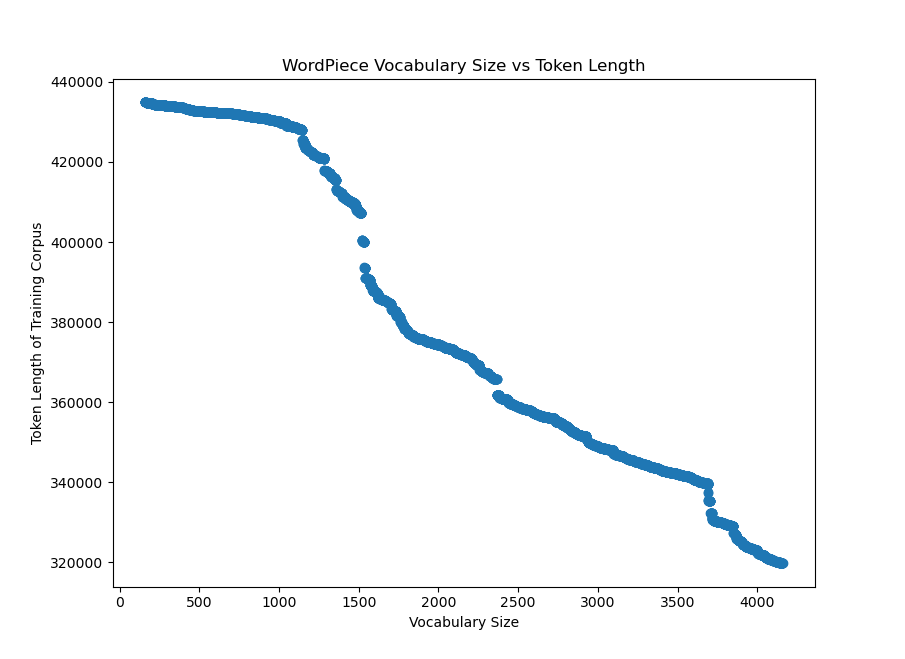
\includegraphics[width=1\textwidth]{../scatter2.png}

                The final vocabulary size after training the WordPiece tokenizer is \textbf{4158} types.
                The total length of the training data under the final type vocabulary is \textbf{319769}.
        \end{answer}
     \end{part}
     

     \begin{part}
        \begin{answer}
            1. Applying the trained WordPiece tokenizer on the last 1000 lines of the dataset gave a total of \textbf{79223} tokens.\\
            2. Tokenized sequence for i): 

            ['A', 'n', 'a', 'l', 'y', 's', 't', 's', 'w', 'e', 'r', 'e', 'expecting', 'the', 'o', 'p', 'p', 'o', 's', 'i', 't', 'e', ',', 'a', 'd', 'e', 'e', 'p', 'e', 'n', 'ing', 'of', 'the', 'd', 'e', 'f', 'i', 'c', 'i', 't', '.']\\

            3. Tokenized sequence for ii): 


            ['Five', 'm', 'i', 'n', 'u', 't', 'e', 's', 'l', 'a', 't', 'e', 'r', ',', 'a', 's', 'e', 'c', 'o', 'nd', 'p', 'e', 'r', 's', 'o', 'n', 'a', 'r', 'r', 'i', 've', 'd', ',', 'a', 'g', 'ed', 'around', 'th', 'i', 'r', 't', 'y,', 'with', 'k', 'n', 'i', 'f', 'e', 'w', 'o', 'u', 'n', 'd', 's', '.']

        \end{answer}
     \end{part}

     \begin{part}
        \begin{answer}
            Assuming that my implementations were correct:\\
            WordPiece seems to be better at preserving coherent semantics, while BPE tends to chop up words into smaller chunks. In the
            two sentences we above the tokens that are more than 2 characters tends to have semantic meanings (e.g. 'nd', 'ing', 'ed', and all the full words).
            This might be good for things like translation where we want to preserve the meaning of the subwords can be important.\\
            On the downside, WordPiece's takes a really long time to build up vocabulary compared to BPE. In my implementation, WordPiece took more than twice the time to build up
            less than half the vocabulary size of BPE (575 sec for vocab size of 4158 vs 215 sec for vocab size of 9124).\\
            So I think BPE might be better for tasks that require a large vocabulary size, such as language modeling, and WordPiece might be better for tasks that require
            a smaller vocabulary size but more semantic information, such as translation.\\

            Tokenized sequence using BPE:\\
            for i): 
            
            ['Analy', 'sts', 'were', 'expect', 'ing', 'the', 'oppos', 'ite,', 'a', 'deep', 'ening', 'of', 'the', 'deficit.'] \\


            for ii): 
            
            ['Five', 'minutes', 'later,', 'a', 'second', 'person', 'arri', 'ved,', 'aged', 'around', 'thir', 'ty,', 'with', 'kni', 'fe', 'wo', 'und', 's.']
        \end{answer}
     \end{part}

\end{question}

%%%%%%%%%%%%%%%%%%%%%%%% Task 5 %%%%%%%%%%%%%%%%%%%%%%%%
\begin{question}{Acknowledgement}
   
    \begin{answer}
        This assignment was completed by Sebastian Liu.
        ChatGPT 3.5 and Github Copilot were used as a human collaborator to:
        \begin{itemize}
            \item Ask conceptual questions about N-gram models, Laplace smoothing, interpolation, BPE, and WordPiece. (e.g. What is perplexity and why it works?)
            \item Ask how-to questions related to python. (e.g. How to use regex in python? How to concatenate any number of strings in python?)
            \item Generate repetitive, long sequences of print statement in experiments. (e.g. calling and print perplexities for different lambda values in interpolation)
        \end{itemize}
    \end{answer}

\end{question}
\end{document}

